\documentclass[11pt,fleqn, oneside,openany]{extbook} % Default font size and left-justified equations

% use this list: https://www.educative.io/blog/google-coding-interview

%%%%%%%%%%%%%%%%%%%%%%%%%%%%%%%%%%%%%%%%%%%%
%               Structure
%%%%%%%%%%%%%%%%%%%%%%%%%%%%%%%%%%%%%%%%%%%%
%%%%%%%%%%%%%%%%%%%%%%%%%%%%%%%%%%%%%%%%%
% The Legrand Orange Book
% Structural Definitions File
% Version 2.0 (9/2/15)
%
% Original author:
% Mathias Legrand (legrand.mathias@gmail.com) with modifications by:
% Vel (vel@latextemplates.com)
% 
% This file has been downloaded from:
% http://www.LaTeXTemplates.com
%
% License:
% CC BY-NC-SA 3.0 (http://creativecommons.org/licenses/by-nc-sa/3.0/)
%
%%%%%%%%%%%%%%%%%%%%%%%%%%%%%%%%%%%%%%%%%

%----------------------------------------------------------------------------------------
%	VARIOUS REQUIRED PACKAGES AND CONFIGURATIONS
%----------------------------------------------------------------------------------------

\usepackage[top=3cm,bottom=3cm,left=3cm,right=3cm,headsep=10pt,a4paper]{geometry} % Page margins

\usepackage{graphicx} % Required for including pictures
\graphicspath{{images/}} % Specifies the directory where pictures are stored

\usepackage{lipsum} % Inserts dummy text

\usepackage{tikz} % Required for drawing custom shapes

\usepackage[english]{babel} % English language/hyphenation

\usepackage{enumitem} % Customize lists
\setlist{nolistsep} % Reduce spacing between bullet points and numbered lists

\usepackage{booktabs} % Required for nicer horizontal rules in tables

\usepackage{xcolor} % Required for specifying colors by name
\definecolor{ocre}{RGB}{243,102,25} % Define the orange color used for highlighting throughout the book

%----------------------------------------------------------------------------------------
%	FONTS
%----------------------------------------------------------------------------------------

\usepackage{avant} % Use the Avantgarde font for headings
%\usepackage{times} % Use the Times font for headings
\usepackage{mathptmx} % Use the Adobe Times Roman as the default text font together with math symbols from the Sym­bol, Chancery and Com­puter Modern fonts

\usepackage{microtype} % Slightly tweak font spacing for aesthetics
\usepackage[utf8]{inputenc} % Required for including letters with accents
\usepackage[T1]{fontenc} % Use 8-bit encoding that has 256 glyphs

%----------------------------------------------------------------------------------------
%	BIBLIOGRAPHY AND INDEX
%----------------------------------------------------------------------------------------

\usepackage[citestyle=numeric,sorting=nyt,sortcites=true,autopunct=true,babel=hyphen,hyperref=true,abbreviate=false,backref=true,backend=biber]{biblatex}
\addbibresource{sources/bibliography.bib}
\defbibheading{bibempty}{}

\usepackage{calc} % For simpler calculation - used for spacing the index letter headings correctly
\usepackage{makeidx} % Required to make an index
\makeindex % Tells LaTeX to create the files required for indexing

%----------------------------------------------------------------------------------------
%	MAIN TABLE OF CONTENTS
%----------------------------------------------------------------------------------------

\usepackage{titletoc} % Required for manipulating the table of contents

\contentsmargin{0cm} % Removes the default margin

% Part text styling
\titlecontents{part}[0cm]
{\addvspace{20pt}\centering\large\bfseries}
{}
{}
{}

% Chapter text styling
\titlecontents{chapter}[1.25cm] % Indentation
{\addvspace{12pt}\large\sffamily\bfseries} % Spacing and font options for chapters
{\color{ocre!60}\contentslabel[\Large\thecontentslabel]{1.25cm}\color{ocre}} % Chapter number
{\color{ocre}}  
{\color{ocre!60}\normalsize\;\titlerule*[.5pc]{.}\;\thecontentspage} % Page number

% Section text styling
\titlecontents{section}[1.25cm] % Indentation
{\addvspace{3pt}\sffamily\bfseries} % Spacing and font options for sections
{\contentslabel[\thecontentslabel]{1.25cm}} % Section number
{}
{\hfill\color{black}\thecontentspage} % Page number
[]

% Subsection text styling
\titlecontents{subsection}[1.25cm] % Indentation
{\addvspace{1pt}\sffamily\small} % Spacing and font options for subsections
{\contentslabel[\thecontentslabel]{1.25cm}} % Subsection number
{}
{\ \titlerule*[.5pc]{.}\;\thecontentspage} % Page number
[]

% List of figures
\titlecontents{figure}[0em]
{\addvspace{-5pt}\sffamily}
{\thecontentslabel\hspace*{1em}}
{}
{\ \titlerule*[.5pc]{.}\;\thecontentspage}
[]

% List of tables
\titlecontents{table}[0em]
{\addvspace{-5pt}\sffamily}
{\thecontentslabel\hspace*{1em}}
{}
{\ \titlerule*[.5pc]{.}\;\thecontentspage}
[]

%----------------------------------------------------------------------------------------
%	MINI TABLE OF CONTENTS IN PART HEADS
%----------------------------------------------------------------------------------------

% Chapter text styling
\titlecontents{lchapter}[0em] % Indenting
{\addvspace{15pt}\large\sffamily\bfseries} % Spacing and font options for chapters
{\color{ocre}\contentslabel[\Large\thecontentslabel]{1.25cm}\color{ocre}} % Chapter number
{}  
{\color{ocre}\normalsize\sffamily\bfseries\;\titlerule*[.5pc]{.}\;\thecontentspage} % Page number

% Section text styling
\titlecontents{lsection}[0em] % Indenting
{\sffamily\small} % Spacing and font options for sections
{\contentslabel[\thecontentslabel]{1.25cm}} % Section number
{}
{}

% Subsection text styling
\titlecontents{lsubsection}[.5em] % Indentation
{\normalfont\footnotesize\sffamily} % Font settings
{}
{}
{}

%----------------------------------------------------------------------------------------
%	PAGE HEADERS
%----------------------------------------------------------------------------------------

\usepackage{fancyhdr} % Required for header and footer configuration

\pagestyle{fancy}
\renewcommand{\chaptermark}[1]{\markboth{\sffamily\normalsize\bfseries\chaptername\ \thechapter.\ #1}{}} % Chapter text font settings
\renewcommand{\sectionmark}[1]{\markright{\sffamily\normalsize\thesection\hspace{5pt}#1}{}} % Section text font settings
\fancyhf{} \fancyhead[LE,RO]{\sffamily\normalsize\thepage} % Font setting for the page number in the header
\fancyhead[LO]{\rightmark} % Print the nearest section name on the left side of odd pages
\fancyhead[RE]{\leftmark} % Print the current chapter name on the right side of even pages
\renewcommand{\headrulewidth}{0.5pt} % Width of the rule under the header
\addtolength{\headheight}{2.5pt} % Increase the spacing around the header slightly
\renewcommand{\footrulewidth}{0pt} % Removes the rule in the footer
\fancypagestyle{plain}{\fancyhead{}\renewcommand{\headrulewidth}{0pt}} % Style for when a plain pagestyle is specified

% Removes the header from odd empty pages at the end of chapters
\makeatletter
\renewcommand{\cleardoublepage}{
\clearpage\ifodd\c@page\else
\hbox{}
\vspace*{\fill}
\thispagestyle{empty}
\newpage
\fi}

%----------------------------------------------------------------------------------------
%	THEOREM STYLES
%----------------------------------------------------------------------------------------


\usepackage{amsmath,amsfonts,amssymb,amsthm,mathtools} % For math equations, theorems, symbols, etc
\DeclarePairedDelimiter\ceil{\lceil}{\rceil}
\DeclarePairedDelimiter\floor{\lfloor}{\rfloor}

\newcommand{\intoo}[2]{\mathopen{]}#1\,;#2\mathclose{[}}
\newcommand{\ud}{\mathop{\mathrm{{}d}}\mathopen{}}
\newcommand{\intff}[2]{\mathopen{[}#1\,;#2\mathclose{]}}
\newtheorem{notation}{Notation}[chapter]

% Boxed/framed environments
\newtheoremstyle{ocrenumbox}% % Theorem style name
{0pt}% Space above
{0pt}% Space below
{\normalfont}% % Body font
{}% Indent amount
{\small\bf\sffamily\color{ocre}}% % Theorem head font
{\;}% Punctuation after theorem head
{0.25em}% Space after theorem head
{\small\sffamily\color{ocre}\thmname{#1}\nobreakspace\thmnumber{\@ifnotempty{#1}{}\@upn{#2}}% Theorem text (e.g. Theorem 2.1)
\thmnote{\nobreakspace\the\thm@notefont\sffamily\bfseries\color{black}---\nobreakspace#3.}} % Optional theorem note
\renewcommand{\qedsymbol}{$\blacksquare$}% Optional qed square

\newtheoremstyle{blacknumex}% Theorem style name
{5pt}% Space above
{5pt}% Space below
{\normalfont}% Body font
{} % Indent amount
{\small\bf\sffamily}% Theorem head font
{\;}% Punctuation after theorem head
{0.25em}% Space after theorem head
{\small\sffamily{\tiny\ensuremath{\blacksquare}}\nobreakspace\thmname{#1}\nobreakspace\thmnumber{\@ifnotempty{#1}{}\@upn{#2}}% Theorem text (e.g. Theorem 2.1)
\thmnote{\nobreakspace\the\thm@notefont\sffamily\bfseries---\nobreakspace#3.}}% Optional theorem note

\newtheoremstyle{blacknumbox} % Theorem style name
{0pt}% Space above
{0pt}% Space below
{\normalfont}% Body font
{}% Indent amount
{\small\bf\sffamily}% Theorem head font
{\;}% Punctuation after theorem head
{0.25em}% Space after theorem head
{\small\sffamily\thmname{#1}\nobreakspace\thmnumber{\@ifnotempty{#1}{}\@upn{#2}}% Theorem text (e.g. Theorem 2.1)
\thmnote{\nobreakspace\the\thm@notefont\sffamily\bfseries---\nobreakspace#3.}}% Optional theorem note

% Non-boxed/non-framed environments
\newtheoremstyle{ocrenum}% % Theorem style name
{5pt}% Space above
{5pt}% Space below
{\normalfont}% % Body font
{}% Indent amount
{\small\bf\sffamily\color{ocre}}% % Theorem head font
{\;}% Punctuation after theorem head
{0.25em}% Space after theorem head
{\small\sffamily\color{ocre}\thmname{#1}\nobreakspace\thmnumber{\@ifnotempty{#1}{}\@upn{#2}}% Theorem text (e.g. Theorem 2.1)
\thmnote{\nobreakspace\the\thm@notefont\sffamily\bfseries\color{black}---\nobreakspace#3.}} % Optional theorem note
\renewcommand{\qedsymbol}{$\blacksquare$}% Optional qed square
\makeatother

% Defines the theorem text style for each type of theorem to one of the three styles above
\newcounter{dummy} 
\numberwithin{dummy}{section}
\theoremstyle{ocrenumbox}
\newtheorem{theoremeT}[dummy]{Theorem}

\newtheorem{problem}{Exercise}[chapter]
\newtheorem{exerciseT}{Problem}
\theoremstyle{blacknumex}
\newtheorem{solution}{Solution}[chapter]
\newtheorem{solutionT}{solution}[chapter]
\theoremstyle{blacknumex}
\newtheorem{exampleT}{Example}[chapter]
\theoremstyle{blacknumbox}
\newtheorem{vocabulary}{Vocabulary}[chapter]
\newtheorem{definitionT}{Definition}[section]
\newtheorem{corollaryT}[dummy]{Corollary}
\theoremstyle{ocrenum}
\newtheorem{proposition}[dummy]{Proposition}

%----------------------------------------------------------------------------------------
%	DEFINITION OF COLORED BOXES
%----------------------------------------------------------------------------------------

\RequirePackage[framemethod=default]{mdframed} % Required for creating the theorem, definition, exercise and corollary boxes

% Theorem box
\newmdenv[skipabove=7pt,
skipbelow=7pt,
backgroundcolor=black!5,
linecolor=ocre,
innerleftmargin=5pt,
innerrightmargin=5pt,
innertopmargin=5pt,
leftmargin=0cm,
rightmargin=0cm,
innerbottommargin=5pt]{tBox}

% Exercise box	  
\newmdenv[skipabove=7pt,
skipbelow=7pt,
rightline=false,
leftline=true,
topline=false,
bottomline=false,
backgroundcolor=ocre!10,
linecolor=ocre,
innerleftmargin=5pt,
innerrightmargin=5pt,
innertopmargin=5pt,
innerbottommargin=5pt,
leftmargin=0cm,
rightmargin=0cm,
linewidth=4pt]{eBox}	

% Definition box
\newmdenv[skipabove=7pt,
skipbelow=7pt,
rightline=false,
leftline=true,
topline=false,
bottomline=false,
linecolor=ocre,
innerleftmargin=5pt,
innerrightmargin=5pt,
innertopmargin=0pt,
leftmargin=0cm,
rightmargin=0cm,
linewidth=4pt,
innerbottommargin=0pt]{dBox}	

% Corollary box
\newmdenv[skipabove=7pt,
skipbelow=7pt,
rightline=false,
leftline=true,
topline=false,
bottomline=false,
linecolor=gray,
backgroundcolor=black!5,
innerleftmargin=5pt,
innerrightmargin=5pt,
innertopmargin=5pt,
leftmargin=0cm,
rightmargin=0cm,
linewidth=4pt,
innerbottommargin=5pt]{cBox}

% Creates an environment for each type of theorem and assigns it a theorem text style from the "Theorem Styles" section above and a colored box from above
\newenvironment{theorem}{\begin{tBox}\begin{theoremeT}}{\end{theoremeT}\end{tBox}}
\newenvironment{exercise}{\begin{eBox}\begin{exerciseT}}{\hfill{\color{ocre}\tiny\ensuremath{\blacksquare}}\end{exerciseT}\end{eBox}}				  
\newenvironment{definition}{\begin{dBox}\begin{definitionT}}{\end{definitionT}\end{dBox}}	
\newenvironment{example}{\begin{exampleT}}{\hfill{\tiny\ensuremath{\blacksquare}}\end{exampleT}}		
\newenvironment{corollary}{\begin{cBox}\begin{corollaryT}}{\end{corollaryT}\end{cBox}}	

%----------------------------------------------------------------------------------------
%	REMARK ENVIRONMENT
%----------------------------------------------------------------------------------------

\newenvironment{remark}{\par\vspace{10pt}\small % Vertical white space above the remark and smaller font size
\begin{list}{}{
\leftmargin=35pt % Indentation on the left
\rightmargin=25pt}\item\ignorespaces % Indentation on the right
\makebox[-2.5pt]{\begin{tikzpicture}[overlay]
\node[draw=ocre!60,line width=1pt,circle,fill=ocre!25,font=\sffamily\bfseries,inner sep=2pt,outer sep=0pt] at (-15pt,0pt){\textcolor{ocre}{R}};\end{tikzpicture}} % Orange R in a circle
\advance\baselineskip -1pt}{\end{list}\vskip5pt} % Tighter line spacing and white space after remark

%----------------------------------------------------------------------------------------
%	SECTION NUMBERING IN THE MARGIN
%----------------------------------------------------------------------------------------

\makeatletter
\renewcommand{\@seccntformat}[1]{\llap{\textcolor{ocre}{\csname the#1\endcsname}\hspace{1em}}}                    
\renewcommand{\section}{\@startsection{section}{1}{\z@}
{-4ex \@plus -1ex \@minus -.4ex}
{1ex \@plus.2ex }
{\normalfont\large\sffamily\bfseries}}
\renewcommand{\subsection}{\@startsection {subsection}{2}{\z@}
{-3ex \@plus -0.1ex \@minus -.4ex}
{0.5ex \@plus.2ex }
{\normalfont\sffamily\bfseries}}
\renewcommand{\subsubsection}{\@startsection {subsubsection}{3}{\z@}
{-2ex \@plus -0.1ex \@minus -.2ex}
{.2ex \@plus.2ex }
{\normalfont\small\sffamily\bfseries}}                        
\renewcommand\paragraph{\@startsection{paragraph}{4}{\z@}
{-2ex \@plus-.2ex \@minus .2ex}
{.1ex}
{\normalfont\small\sffamily\bfseries}}

%----------------------------------------------------------------------------------------
%	PART HEADINGS
%----------------------------------------------------------------------------------------

% numbered part in the table of contents
\newcommand{\@mypartnumtocformat}[2]{%
\setlength\fboxsep{0pt}%
\noindent\colorbox{ocre!20}{\strut\parbox[c][.7cm]{\ecart}{\color{ocre!70}\Large\sffamily\bfseries\centering#1}}\hskip\esp\colorbox{ocre!40}{\strut\parbox[c][.7cm]{\linewidth-\ecart-\esp}{\Large\sffamily\centering#2}}}%
%%%%%%%%%%%%%%%%%%%%%%%%%%%%%%%%%%
% unnumbered part in the table of contents
\newcommand{\@myparttocformat}[1]{%
\setlength\fboxsep{0pt}%
\noindent\colorbox{ocre!40}{\strut\parbox[c][.7cm]{\linewidth}{\Large\sffamily\centering#1}}}%
%%%%%%%%%%%%%%%%%%%%%%%%%%%%%%%%%%
\newlength\esp
\setlength\esp{4pt}
\newlength\ecart
\setlength\ecart{1.2cm-\esp}
\newcommand{\thepartimage}{}%
\newcommand{\partimage}[1]{\renewcommand{\thepartimage}{#1}}%
\def\@part[#1]#2{%
\ifnum \c@secnumdepth >-2\relax%
\refstepcounter{part}%
\addcontentsline{toc}{part}{\texorpdfstring{\protect\@mypartnumtocformat{\thepart}{#1}}{\partname~\thepart\ ---\ #1}}
\else%
\addcontentsline{toc}{part}{\texorpdfstring{\protect\@myparttocformat{#1}}{#1}}%
\fi%
\startcontents%
\markboth{}{}%
{\thispagestyle{empty}%
\begin{tikzpicture}[remember picture,overlay]%
\node at (current page.north west){\begin{tikzpicture}[remember picture,overlay]%	
\fill[ocre!20](0cm,0cm) rectangle (\paperwidth,-\paperheight);
\node[anchor=north] at (4cm,-3.25cm){\color{ocre!40}\fontsize{220}{100}\sffamily\bfseries\@Roman\c@part}; 
\node[anchor=south east] at (\paperwidth-1cm,-\paperheight+1cm){\parbox[t][][t]{8.5cm}{
\printcontents{l}{0}{\setcounter{tocdepth}{1}}%
}};
\node[anchor=north east] at (\paperwidth-1.5cm,-3.25cm){\parbox[t][][t]{15cm}{\strut\raggedleft\color{white}\fontsize{30}{30}\sffamily\bfseries#2}};
\end{tikzpicture}};
\end{tikzpicture}}%
\@endpart}
\def\@spart#1{%
\startcontents%
\phantomsection
{\thispagestyle{empty}%
\begin{tikzpicture}[remember picture,overlay]%
\node at (current page.north west){\begin{tikzpicture}[remember picture,overlay]%	
\fill[ocre!20](0cm,0cm) rectangle (\paperwidth,-\paperheight);
\node[anchor=north east] at (\paperwidth-1.5cm,-3.25cm){\parbox[t][][t]{15cm}{\strut\raggedleft\color{white}\fontsize{30}{30}\sffamily\bfseries#1}};
\end{tikzpicture}};
\end{tikzpicture}}
\addcontentsline{toc}{part}{\texorpdfstring{%
\setlength\fboxsep{0pt}%
\noindent\protect\colorbox{ocre!40}{\strut\protect\parbox[c][.7cm]{\linewidth}{\Large\sffamily\protect\centering #1\quad\mbox{}}}}{#1}}%
\@endpart}
\def\@endpart{\vfil\newpage
\if@twoside
\if@openright
\null
\thispagestyle{empty}%
\newpage
\fi
\fi
\if@tempswa
\twocolumn
\fi}

%----------------------------------------------------------------------------------------
%	CHAPTER HEADINGS
%----------------------------------------------------------------------------------------

% A switch to conditionally include a picture, implemented by  Christian Hupfer
\newif\ifusechapterimage
\usechapterimagetrue
\newcommand{\thechapterimage}{}%
\newcommand{\chapterimage}[1]{\ifusechapterimage\renewcommand{\thechapterimage}{#1}\fi}%
\def\@makechapterhead#1{%
{\parindent \z@ \raggedright \normalfont
\ifnum \c@secnumdepth >\m@ne
\if@mainmatter
\begin{tikzpicture}[remember picture,overlay]
\node at (current page.north west)
{\begin{tikzpicture}[remember picture,overlay]
\node[anchor=north west,inner sep=0pt] at (0,0) {\ifusechapterimage\includegraphics[width=\paperwidth]{\thechapterimage}\fi};
\draw[anchor=west] (\Gm@lmargin,-4cm) node [line width=2pt,rounded corners=15pt,draw=ocre,fill=white,fill opacity=0.5,inner sep=15pt]{\strut\makebox[22cm]{}};
\draw[anchor=west] (\Gm@lmargin+.3cm,-4cm) node {\huge\sffamily\bfseries\color{black}\thechapter. #1\strut};
\end{tikzpicture}};
\end{tikzpicture}
\else
\begin{tikzpicture}[remember picture,overlay]
\node at (current page.north west)
{\begin{tikzpicture}[remember picture,overlay]
\node[anchor=north west,inner sep=0pt] at (0,0) {\ifusechapterimage\includegraphics[width=\paperwidth]{\thechapterimage}\fi};
\draw[anchor=west] (\Gm@lmargin,-4cm) node [line width=2pt,rounded corners=15pt,draw=ocre,fill=white,fill opacity=0.5,inner sep=15pt]{\strut\makebox[22cm]{}};
\draw[anchor=west] (\Gm@lmargin+.3cm,-4cm) node {\huge\sffamily\bfseries\color{black}#1\strut};
\end{tikzpicture}};
\end{tikzpicture}
\fi\fi\par\vspace*{100\p@}}}

%-------------------------------------------

\def\@makeschapterhead#1{%
\begin{tikzpicture}[remember picture,overlay]
\node at (current page.north west)
{\begin{tikzpicture}[remember picture,overlay]
\node[anchor=north west,inner sep=0pt] at (0,0) {\ifusechapterimage\includegraphics[width=\paperwidth]{\thechapterimage}\fi};
\draw[anchor=west] (\Gm@lmargin,-4cm) node [line width=2pt,rounded corners=15pt,draw=ocre,fill=white,fill opacity=0.5,inner sep=15pt]{\strut\makebox[22cm]{}};
\draw[anchor=west] (\Gm@lmargin+.3cm,-4cm) node {\huge\sffamily\bfseries\color{black}#1\strut};
\end{tikzpicture}};
\end{tikzpicture}
\par\vspace*{100\p@}}
\makeatother

%----------------------------------------------------------------------------------------
%	HYPERLINKS IN THE DOCUMENTS
%----------------------------------------------------------------------------------------

\usepackage{hyperref}
\hypersetup{hidelinks,backref=true,pagebackref=true,hyperindex=true,colorlinks=false,breaklinks=true,urlcolor= ocre,bookmarks=true,bookmarksopen=false,pdftitle={Title},pdfauthor={Author}}
\usepackage{bookmark}
\bookmarksetup{
open,
numbered,
addtohook={%
\ifnum\bookmarkget{level}=0 % chapter
\bookmarksetup{bold}%
\fi
\ifnum\bookmarkget{level}=-1 % part
\bookmarksetup{color=ocre,bold}%
\fi
}
}

%----------------------------------------------------------------------------------------
%	LISTINGS
%----------------------------------------------------------------------------------------
%----------------------------------------------------------------------------------------
%	LISTINGS
%----------------------------------------------------------------------------------------
\usepackage{listings}
\lstset{language=C++}
\lstset{
	basicstyle=\footnotesize\ttfamily,
	breaklines=true,
	showstringspaces=false,
	numbers=left,
	backgroundcolor=\color{bgcolor},
	commentstyle=\color{gray},
	keywordstyle=\color{blue},
	keywordstyle=[2]\color{teal},   % cyan or teal can also be a good choice, use \bfseries for bold
	frame=none,                     % adds a frame around the code
	tabsize=2,                      % sets default tabsize to 2 spaces
	captionpos=b,                   % sets the caption-position to bottom
	morekeywords=[2]{}              % if you want to add more keywords to the set
	__
}

\definecolor{mygreen}{RGB}{28,172,0} % color values Red, Green, Blue
\definecolor{mylilas}{RGB}{170,55,241}
\lstset{language=Matlab,%
    %basicstyle=\color{red},
    breaklines=true,%
    morekeywords={matlab2tikz},
    keywordstyle=\color{blue},%
    morekeywords=[2]{1}, keywordstyle=[2]{\color{black}},
    identifierstyle=\color{black},%
    stringstyle=\color{mylilas},
    commentstyle=\color{mygreen},%
    showstringspaces=false,%without this there will be a symbol in the places where there is a space
    numbers=left,%
    numberstyle={\tiny \color{black}},% size of the numbers
    numbersep=9pt, % this defines how far the numbers are from the text
    emph=[1]{for,end,break},emphstyle=[1]\color{red}, %some words to emphasise
    %emph=[2]{word1,word2}, emphstyle=[2]{style},    
}

\usepackage{color}
\definecolor{bgcolor}{rgb}{0.98,0.98,0.98}


%----------------------------------------------------------------------------------------

%	QandA

%----------------------------------------------------------------------------------------

\newenvironment{QandA}{\begin{enumerate}[label=\bfseries Q.\arabic*.,leftmargin=2em,rightmargin=2em]\bfseries}{\end{enumerate}}
\newenvironment{answered}{\par\normalfont}{}
%----------------------------------------------------------------------------------------
%	ALGORITHM
%----------------------------------------------------------------------------------------
\usepackage[]{algorithm2e}

\RestyleAlgo{boxruled}
\usepackage{mdframed,framed}

\SetKwProg{Fn}{Function}{}{}
\SetKwRepeat{Do}{do}{while}%
\SetKwFunction{CreateHashSet}{CreateHashSet<int>}


\DeclarePairedDelimiter\abs{\lvert}{\rvert}%
\DeclarePairedDelimiter\norm{\lVert}{\rVert}%

% Swap the definition of \abs* and \norm*, so that \abs
% and \norm resizes the size of the brackets, and the 
% starred version does not.
\makeatletter
\let\oldabs\abs
\def\abs{\@ifstar{\oldabs}{\oldabs*}}
%
\let\oldnorm\norm
\def\norm{\@ifstar{\oldnorm}{\oldnorm*}}
\makeatother

\usepackage[makeroom]{cancel}


\interfootnotelinepenalty=10000

\begin{document}

%\frontmatter
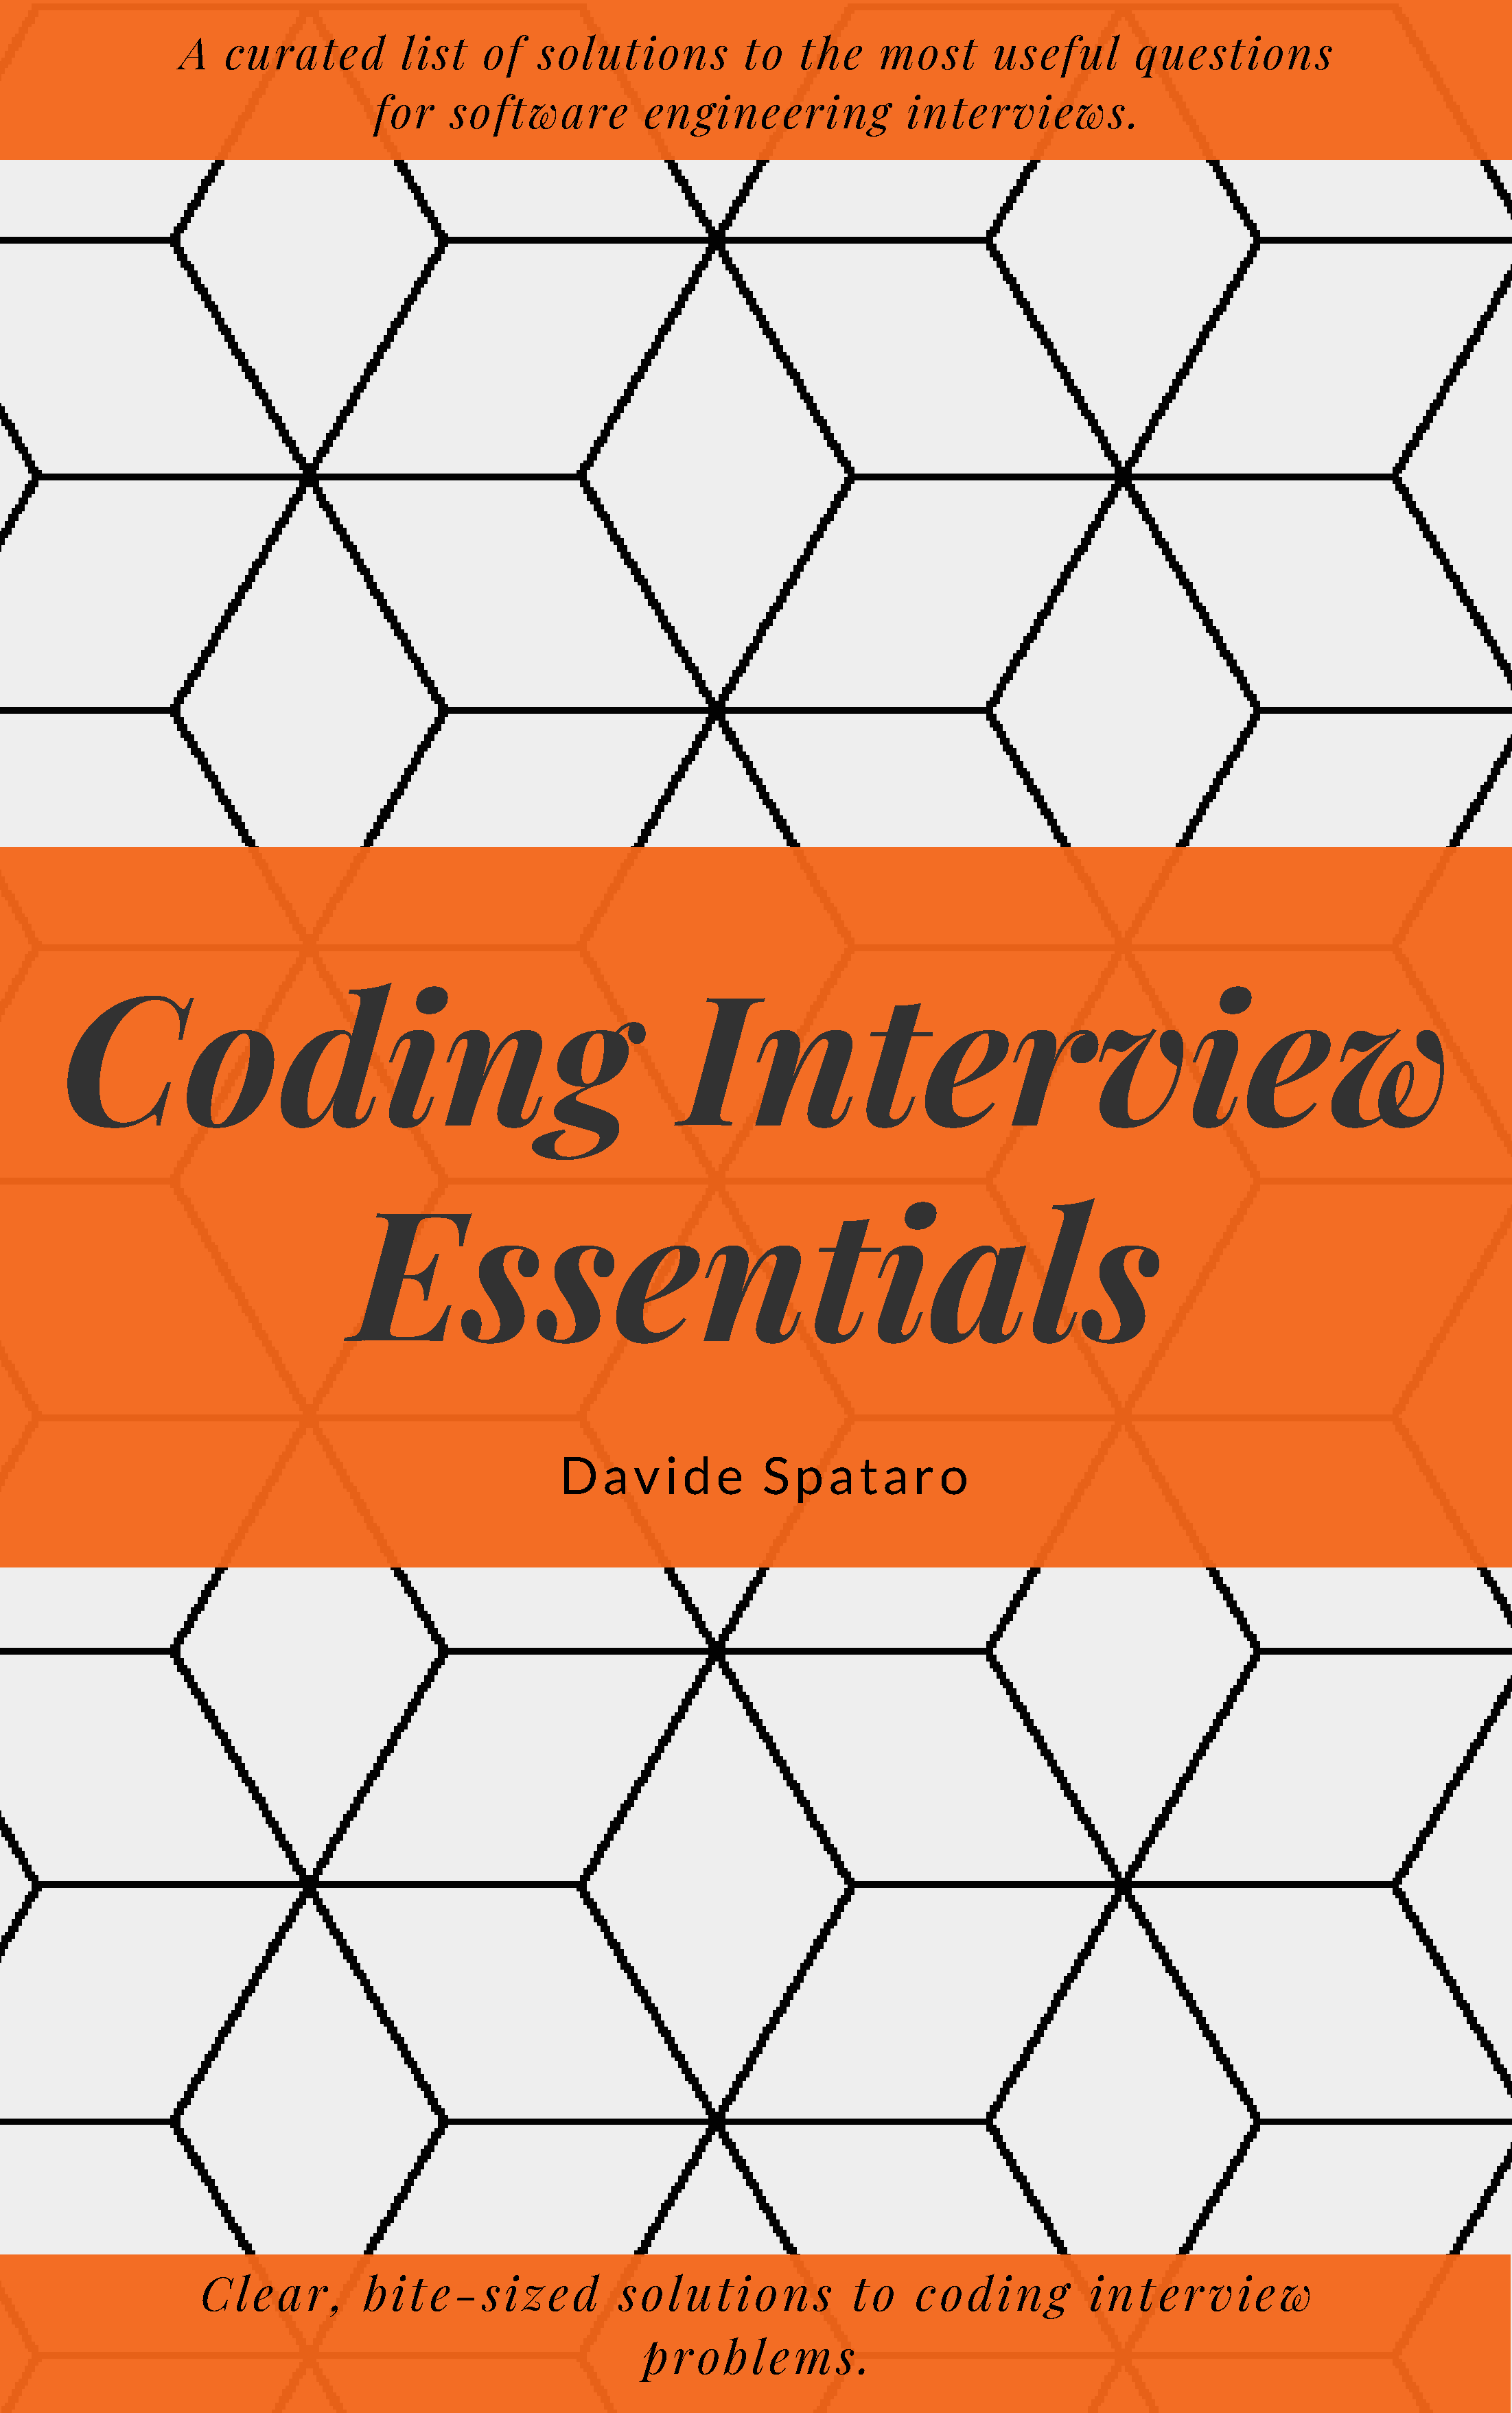
\includepdf[pages=1, fitpaper]{sources/front_cover_image.pdf}
%%\begingroup
%\thispagestyle{empty}
%\begin{tikzpicture}[remember picture,overlay]
%  \coordinate [below=12cm] (midpoint) at (current page.north);
%  \node at (current page.north west)
%  {\begin{tikzpicture}[remember picture,overlay]
%      \node[anchor=north west,inner sep=0pt] at (0,0) {
\includegraphics[width=\paperwidth]{images/background}}; % Background image
%\textsl{}
%      \draw[anchor=north] (midpoint) node [fill=ocre!30!white,fill opacity=0.6,text opacity=1,inner sep=1cm]{\Huge\centering\bfseries\sffamily\parbox[c][][t]{\paperwidth}{\centering Coding Interview Essentials\\[15pt] % Book title
%      {\Large - }\\[20pt] % Subtitle
%      {\huge Davide Spataro}}}; % Author name
%    \end{tikzpicture}};
%\end{tikzpicture}
%\vfill
%\endgroup


\includepdf[pages={2},fitpaper=true]{images/book_covers1.pdf}


\usechapterimagefalse % If you don't want to include a chapter image, use this to toggle images off - it can be enabled later with \usechapterimagetrue

%\chapterimage{images/header} % Table of contents heading image

\pagestyle{empty} % No headers

\tableofcontents % Print the table of contents itself

%\lstlistoflistings
%\listoffigures
%\listoftables

\cleardoublepage % Forces the first chapter to start on an odd page so it's on the right

%pagestyle{fancy} % Print headers again
%!TEX root = ../main.tex
%%%%%%%%%%%%%%%%%%%%%%%%%%%%%%%%%%
% Links:
%
% Difficulty: Companies: 
%%%%%%%%%%%%%%%%%%%%%%%%%%%%%%%%%%

\chapter{Jump Game}
\label{ch:can_jump}
\section*{Introduction}
In this chapter, we will investigate whether a solution exists for a game played in an array
where you are the only player and you are initially located at the first cell of the array. Your goal is to
get to the last cell by jumping from one cell to another a specified number of times. The array contains
information about the length of the jump you can take from a cell. 

There are several possible different solutions to this problem and, in this Chapter, we will discuss the most common. 
In particular:
\begin{itemize}
    \item In Section \ref{can_jump:sec:backtracking} we take a look at the most intuitive approach where we try all possible jumps in a backtracking-like manner;
    \item In Section \ref{can_jump:sec:DFS} we will refine the solution of Section
    \ref{can_jump:sec:backtracking} into one that uses a clever insight to visit the
    cells efficiently. 
    \item Finally, in Section \ref{can_jump:sec:greedy} we will discuss an efficient and concise
    greedy solution.
\end{itemize}


\section{Problem statement}
\label{ch:can_jump:statement}
\begin{exercise}
Write a function that takes as input an array $I$ of non-negative integers. You are initially
positioned at the beginning of the array (at index $0$) and your goal is to jump from cell to cell
to the end of the array (cell $|I|-1$).
Each cell $i$ of the array contain the maximum lenght for a jump that can be made from cell $i$.
If you are at index $j$ you are allowed to jump to any cell within the following range: $[j-I_i,j+I_i]$.
The function should return true if you can reach the last cell of the array, otherwise it should returns false.

    \begin{example}
        \hfill \\
        Given  $I=[2,3,1,1,4]$ the function returns \textbf{true}. You jump from cell $0$ to $1$ and
        then take a $3$ cells wide jump to the end of the array. See Figure
        \ref{fig:can_jump:example1}.
        \label{ex:can_jump_example1}
    \end{example}

    \begin{example}
        \hfill \\
        Given $I=[3,2,1,0,4]$ the function returns \textbf{false} because it is impossible to reach
        any cells with index higher than $3$. See Figure \ref{fig:can_jump:example2}: there is no
        incoming edge for the node with label $4$.
        \label{ex:can_jump_example2}
    \end{example}
\end{exercise}

\begin{figure}
    \centering
    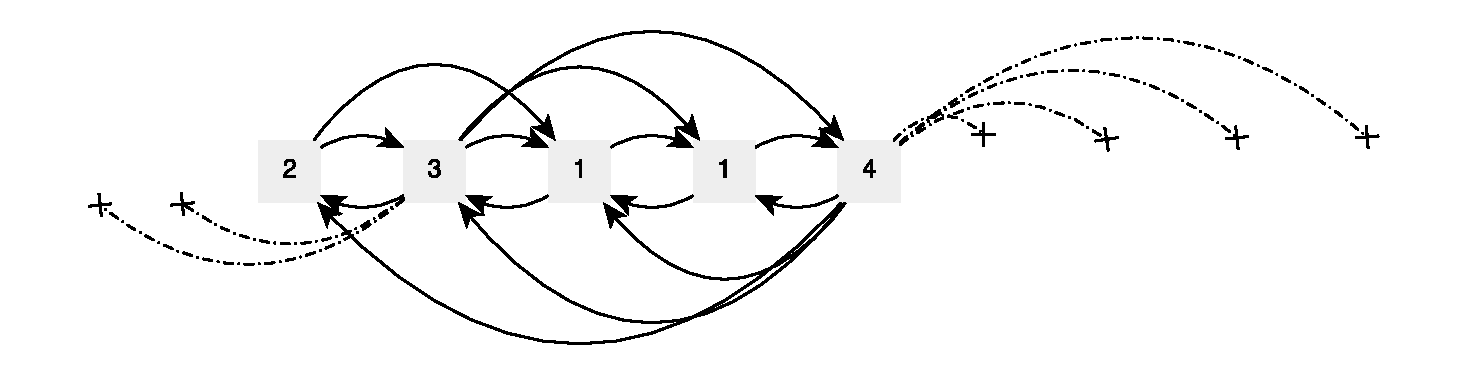
\includegraphics[width=\textwidth]{sources/can_jump/images/can_jump_example1}
    \caption[Implicit graph for the Example \ref{ex:can_jump_example1}.]
    {Visual representation (implicit graph) of the problem instance of Example
    \ref{ex:can_jump_example1}.}.
    \label{fig:can_jump:example1}
\end{figure}

\begin{figure}
    \centering
    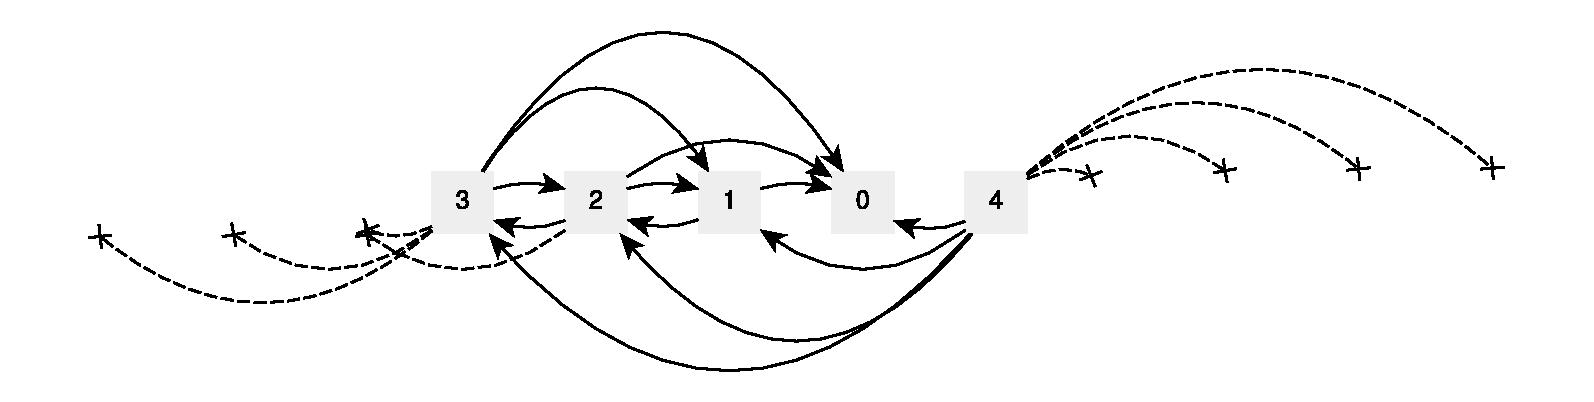
\includegraphics[width=\textwidth]{sources/can_jump/images/example2}
    \caption[Implicit graph for the Example \ref{ex:can_jump_example2}.]
    {Visual representation (implicit graph) of the problem instance of Example
    \ref{ex:can_jump_example2}.}.
    \label{fig:can_jump:example2}
\end{figure}

%\section{Clarification Questions}

%\begin{QandA}
    %\item \begin{answered}
        %\textit{}
    %\end{answered} \end{questionitem}
    
%\end{QandA}

\section{Backtracking}
\label{can_jump:sec:backtracking}
The first solution that we will investigate is based on an idea similar to the DFS where $I$
is treated as an implicit graph where each cell can be thought of as being a node of a graph and is connected to all the others cells that can be
reached by jumping from it.
The set of cells you can reach from a given cell $c$ is identified by
the length of the jump you can perform from $c$ (value that is stored within $c$ itself).
The idea is to use DFS to check whether the last node of the graph is connected with the first one.
In other words, we want to answer to the following question: is there a path from the first to the last node?

We can proceed by adopting a recursive approach where we try to visit all the nodes that we can reach from the node we currently
occupy and to continue this process until either we have reached the last node or there is no more
jump to try; in the latter case,  there is no way to reach the last node (i.e. the last node is
disconnected). 

As the implicit graph is not guaranteed to be acyclic, to make this
approach work we need to ensure that we not jump back and forth from one cell to another in a
cycle. 
This can happen if, for instance,  you jump from a cell $0$ to cell $1$ and then back to cell
$0$. To overcome this issue, we can only perform forward jumps so that it will be impossible
to be stuck in a cycle.
When you jump to a cell $i$ from a cell $j$ s.t. $j < i$ (you performed a forward jump) we know that we can also visit all cells $ j \leq
k \leq i$ (all the cells in between $j$ and $i$) from $j$.
If we only jump forward, we are not going to need to visit any cell $ j \leq k \leq i$ using backward jumps as these cells are visited anyway when processing
cells $j$ by performing forward jumps from it.

An implementation of this idea is shown in Listing
\ref{list:can_jump1_1}. 
This approach is correct and it will eventually find a solution but it is
extremely inefficient. Its complexity is exponential in time as potentially the same cells are
visited over and over\footnote{Suppose $W(x)$ is the number of possible ways you can jump from
position $x$ to the end of the array at index $N$. We know that $T(N) = 1$ (the only way to jump
from cell $N$ to itself is not to jump at all). For all other cells we have that:
    \begin{align*}
        W(x) = \sum_{i=x+1}^N W(i) \\
         = W(x+1) + \sum_{i=x+2}^N W(i) \\
         = W(x+1) + W(x+1) \\
      \end{align*}
    So to calculate $W(X)$ we need the values  $W(x+1)$ twice. The recursive tree for
    $W$ is binary and complete and has height $N$ and therefore contains $O(2^N)$ number of nodes.}
    and constant in space\footnote{if we do not consider the spaces utilized by the stack frames
    during the recursive calls, otherwise it is linear}.

    \lstinputlisting[language=c++, caption={Exponential time solution to the \textit{jump game} problem where only forward jumps are performed.},label=list:can_jump1_1]{sources/can_jump/can_jump_solution1_1.cpp}
 
\section{DFS}
\label{can_jump:sec:DFS}
Another option for solving the cycle problem arising from the algorithm described in Section
\ref{can_jump:sec:backtracking} (this solution can be in-fact thought of as optimized backtracking)
is to keep track of the cells that we have already visited and every time we are about to perform a
jump to a cell we first check whether that cell has already been visited and  - if it has - 
the jump is discarded and not performed. As such, no cell is visited twice and consequently the complexity is in this case is $O(|I|^2)$. In the worst-case scenario you must check for each
cell whether all the other cells have been already visited. Listing \ref{list:can_jump1} shows an
implementation of this idea. 


\lstinputlisting[language=c++, caption={Quadratic time and linear space DFS solution to the \textit{jump game} problem using a visited array.},label=list:can_jump1]{sources/can_jump/can_jump_solution1.cpp}

Note that one optimization from which this solution (and perhaps also Listing
\ref{list:can_jump1_1}) can benefit would be to always try to jump the longest distance possible.
Although this won't change their asymptotic complexity in practice it might be faster.


\section{Greedy}
\label{can_jump:sec:greedy}
There is, however, a much faster solution to this problem using the idea that we can return
true if we can jump from the cell at index $0$ to a cell from which we can reach the end of the
array. If we apply the same reasoning to generic index $i$ we end up with what is essentially a dynamic
programming approach that -  given $G(x)$ is $1$ if you can reach the end of the array from the cell
$x$ and $0$ otherwise - is based on the following recursive formula:
\begin{equation}
    \begin{cases}
        G(|I|-1) = 1 \\
        G(x) = 1 \: \: \text{if} \: \: \exists \: y > x \:\: \text{s.t.} \:\: y < (x+I_x) \: \: \text{and} \: \:G(y) = 1\\
        \text{otherwise} \: \: G(x) = 0
     \end{cases}
    \label{eq:can_jump:dpformula}
\end{equation}
Equation \ref{eq:can_jump:dpformula} shows that a possible implementation would start processing
cells from the last to the first and that for each element a linear time lookup for a suitable cell
$y$ might be needed. Therefore the complexity of this solution is quadratic in time. However we can
drastically lower its complexity by noting that when processing cell $x$ all we care about is
whether the closest cell to the right from which you can reach the end of the array is reachable
from $x$. We can carry this information into a variable $m$ down from cell $|I|-1$ to cell $0$ and
update it after a cell is processed and this would effectively allow us to have a linear time
solution.

To summarize,  the linear time solution for this problem works as follows: We iterate the array $I$
right-to-left and for each cell $x$ we check whether we can reach $m$ jumping from $x$. If we can
then $x$ is the new leftmost cell from which we can reach the end of the array, thus $m = x$.
Otherwise we continue by processing cell $x-1$ in a similar manner. Eventually, we will have
processed all cells and therefore we can return true if $m = 0$ meaning that cell $0$ is the
leftmost cell from which we can jump to location $|I|-1$, and false otherwise.
\lstinputlisting[language=c++, caption={Greedy solution where we use the fact that the DP solution described by Equation \ref{eq:can_jump:dpformula} can be optimized if we only consider if it is possible to reach the closest cell from which we can jump to the end of the array. },label=list:can_jump]{sources/can_jump/can_jump_solution2.cpp}


\section{Jump Game 2}

\section{Problem statement}
\label{can_jump1:sec:statement}
\begin{exercise}
    Given an array of non-negative integers $I$, you are initially positioned at the first index of the array.
    Each element in the array represents your maximum jump length at that position.
    Your goal is to reach the last index in the minimum number of jumps.    
    
    \textbf{You can assume that you can always reach the last index.}
    \begin{example}
        \hfill \\
        Given  $I=[2,3,0,1,4]$ the function returns \textbf{2}. You jump from cell $0$ to $1$ and
        then take a $3$ cells wide jump to the end of the array. See Figure
        \ref{fig:can_jump:example1}.
        \label{ex:can_jump2_example1}
    \end{example}
\end{exercise}

\subsection{Discussion}
The key difference this variation has w.r.t. the version in Section \ref{ch:can_jump:statement} is that here we are guaranteed that it is possible to reach the last location of the array by starting from the beginning and performing some combination of forward jumps. 

When performing the first jump, we know we can reach cells in the range $[0,0+I[0]]$. Which of this cell we should jump to?
The answer is, always jump to the cell at index $j$ in $[0,0+I[0]]$ that get us the farthest! In other words choose the cell $j$ s.t. $j+I[j]$ is maximum.
Why is this the case? 
The reasoning behind it is that, jumping to any other cell other $j$, say cell $0 \leq k \leq 0+I[0]$ with $k \neq j$ does not decrease the overall number of steps to get to the final cell because from cell $j$ we can reach every cell we can reach from cell $k$ plus potentially some more cells that are unreachable from cell $j$.
For example let's examine Figure \ref{fig:can_jump:can_jump2_example1}. Among all the cells we can reach from cells $0$ (in (\textcolor{red}{red}) the cell at index $1$ is the one though which we can travel the farthest. If we decide to jump at cell at index $2$ nothing would change as we would not be able to reach more cells than the ones we can reach from the cell at index $1$.

\begin{figure}
    \centering
    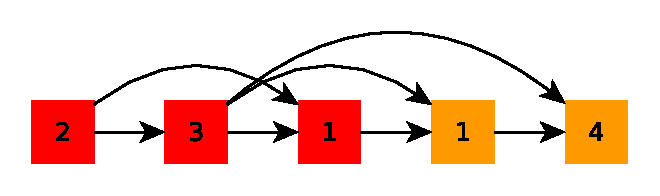
\includegraphics[width=\textwidth]{sources/can_jump/images/can_jump2_example1}
    \caption[]{An instance of the problem with cells divided by color into their respective levels.}.
    \label{fig:can_jump:can_jump2_example1}
\end{figure}

Another way of looking at this problem is by thinking of the cells in being divided in levels and to solve this problem we need to apply a BFS visit to the cells. 
The cells in the interval $[0,I[0]]$ would belong to level $0$. Level $1$ cells would consist of all cells not in level $0$ and that can be reached from any cell of level $0$. 
In general, cells in level $i$ are cells that are not in level $i-1$ and can be reached by jumping from a cell at level $i-1$.
using this definition is it easier to see how the cell that jump the farthest at level $i-1$ would be able to reach all cells of level $i$! There is no other cell in level $i-1$ from which we can reach more cells at the next level.
Therefore, the min number of jumps necessary is equivalent to the level of the last cell.


An implementation of this idea is shown in Listing \ref{list:can_jumps2_1}.


\lstinputlisting[language=c++, caption={Quadratic time and linear space DFS solution to the \textit{jump game} problem using a visited array.},label=list:can_jumps2_1]{sources/can_jump/can_jump2_solution1.cpp}


\section{Jump Game 3}
\label{can_jump3:sec:statement}
\begin{exercise}
    You are given an array of non-negative integers $I$ of size $n$ representing jump lengths and a start position $s$.
    You are initially located at the start index ($0$) of the array. 
    When you are at index $i$, you can jump to index $i + I[i]$ or $i - I[i]$.

    Write a function that given such an array $I$ and start position $s$ returns true if you can reach a cell of $I$ containing the value $0$ and false otherwise by performing 
    zero or more jump starting from $s$.
            
    \textbf{Clearly, you can not jump outside of the array at any time.}
    
    \begin{example}
        \hfill \\
        Given  $I=[4,2,3,0,3,1,2]$ and $s=5$ the function returns \textbf{true}.
        One way to reach cell at index $3$ is by starting from index $5$, then jump to cell $4$, then to cell $1$ and finally to cell $3$.
        \label{ex:can_jump3_example1}
    \end{example}

    \begin{example}
        \hfill \\
        Given  $I=[3,0,2,1,2]$ and $s=2$ the function returns \textbf{false}.
        There is no combination of jumps you can make that will ever make you land at index $1$.
        \label{ex:can_jump3_example2}
    \end{example}
\end{exercise}

\subsection{Discussion}
In the previous variation of this problem discussed in Sections \ref{can_jump1:sec:statement} and \ref{can_jump3:sec:statement} we were allowed to jump from index $i$ to \textbf{any} any cell in the range $[i-I[i],i+I[i]]$, but the variation discussed in this section adds a constraints that forces each jump to be in either of the following two locations:
\begin{itemize}
    \item $i-I[i]$
    \item $i+I[i]$
\end{itemize}.
Another difference is that our target destination is not the end of the array and we will be happy to land in any cell containing a $0$.

In our opinion these contraints do not add significant complexity to the problem as at a closer look, like for the other variation, we are dealing with a graph problem where we are asked to check whether we can reach a certain node.
In general, to be able to reach a node $v$ from another node $u$, we need for $v$ and $u$ to be connected: there must be a path you can take (a serie of jumps in this case) that take you from node $v$ to node $u$.
This condition is easibly checkable by performing a DFS or BFS from node $u$.
For this problem, we are not really interested in a particular node $v$, and provided it contains the value $0$ we are happy.

Therefore we can reframe the problem and ask ourselves whethere exist a node with value $0$ in it that is connected to node $s$. 
This problem is not particularly difficult as all is necessary is to to start a visit of the graph from the node $s$ and stop as soon as either of the following is true:
\begin{itemize}
    \item we have landed to a node with value $0$;
    \item we have visited every node reachable from $s$ (every node in the connected component of $s$).
\end{itemize}
If the first condition is true, then we can stop the visit and return true as we have indeed managed to find a way to jump from $s$ to a node with value $0$ in it; otherwise we can return false, because we have visited every possible node reachable from $s$, but none of them is of the type we want.

Listing \ref{list:can_jumps3_1} shows a possible implementation of this idea.

\lstinputlisting[language=c++, caption={DFS solution.},label=list:can_jumps3_1]{sources/can_jump/can_jump3_solution1.cpp}

The code is nothing more than a simple DFS implementation on the implicit $|I|$ nodes and edges defined by the content of $I$ and the jump rules of the problem statement (from each node $i$ there are at most two edges to nodes at indices $i-I[i]$ and $i+I[i]$, respectively).
Notice that the implicit graph is not guaranteed to be acyclic and some care needs to be taken in order not to visit the same node twice. This is taken care by the \inline{visited} vector of bools, where we store the infomation on whether a node has been visited already.

The time complexity of Listing \ref{list:can_jumps3_1} is $O(|I|)$ (the the number of edges in the implicit graph is also proportional to $|I|$ as each node can have at most two outgoing edges). Its space complexity is likewise linear in the size of $I$.

Finally, notice that if we knew already that a cell in $I$ can ever have a certain value (for instance because we are told that each element of the input array is non-negative) then we could use $I$ itself to mark a cell as visited, thus lowering to space complexity to constant.

%%%%%%%%%%%%%%%%%%%%%%%%%%%%%%%%%%%%%%%%%%%%
%               Appendices
%%%%%%%%%%%%%%%%%%%%%%%%%%%%%%%%%%%%%%%%%%%%

\chapter{Appendices}
%% @Author: Davide Spataro
% @Date:   2020-10-25 
% @Last Modified by:   Davide Spataro
% https://www.topcoder.com/community/competitive-programming/tutorials/dynamic-programming-from-novice-to-advanced/
% file:///home/knotman/Downloads/DYNAMIC_PROGRAMMING_-_ITS_PRINCIPLES_APPLICATIONS_.pdf
% http://smo.sogang.ac.kr/doc/bellman.pdf 
\section*{Dynamic Programming}
\label{sect:appendix:DP}

Dynamic programming (DP) is a popular technique for solving a certain class of
optimization problems efficiently and is accredited to the American Scientist
Richard Bellman\cite{bellman1954}. He conied the term DP in the context of
solving problems involving a serie of best decision one after the other. 
The word \textit{programming} can be a bit deceiving for
computer scientist of programmers in general but it has really little to do with
computer programming and it is infact intended as a set of rules to 
follow to solve a certain problem and it is refeered specifically to the
solution to find an optimal military schedule for logistics (and has more or
less the same meaning as linear programming or linear optimization).  These rules can of course be coded and
executed by a computer but can be easily followed on paper for instance. 
Dynamic programming is better thought as an optimization approach rather than an
method or framework where a complex optimization problem is transformed into a sequence of
smaller (and simpler) problems. The very essence of DP is its multi-stage
optimization procedure. DP does not provide directly with the
instruction on how to solve a particular problem, but instead provides a general
framework that requires creativity and non trivial effort/insights so that a
problem formulation can be adapted and casted within the DP framework bounds.
This is possibly the reason why DP is considered a rather hard topic and it is
particularly feared during interviews. 

This chapter is not intended to be a full treatement of DP, and we will
introduce and describe it to the level that is necessary to understand and
better tackle DP interview problems. For a more comprenshive material on DP
please refer to \cite{bellman1954, cormen2009}.

The gist of the DP approach is that we aim at breaking down a problem into
simpler sub-problems recursively. If it is possible to do so, then the problem
at hand is said to have the \textbf{optimal substructure} property i.e. it can
be solved by using optimal solution to subproblems. But having the optimal
substructure property alone is not enough to prefer a DP approach to another
when trying to solve the same problem. This is because DP really shines when a
problem also exposes the \textbf{overlapping subproblems} property i.e. when the
subproblems are reused several times. A classic example if the
Fibonacci Sequence. In order to calculate $F(n)$ we need to solve two subproblems:
$F(n-1)$ and $F(n-2)$ and adding them up. But for solving $F(n-1)$ we need to
solve $F(n-2)$ \textbf{again}. The value for the subproblem $F(n-2)$ is thus
reused and this makes the Fibonacci problem exposed the optimal substructure
property. 
Dynamic programming takes care of this fact by making sure of solving each
subproblem only once. Usually this can be achieved into two ways:
\begin{description}
    \item [Top-down] This is usually the easiest of the two, by being a direct
    derivation from the recursive formulation of the problem. If the problem can
    be formulated recursively in terms of solution then solution to subproblems
    can be \textit{memoized}\footnote{From the latin word \textit{memorandum}
    which means to be remembered. It is basically a way of remembering the
    result of a function for a certain set of inputs call by storing it in a
    cache.} in a cache. 
    When a subproblem is reused then the
    (potentially expensive) recursive call is avoided and the cached result is
    returned instead. 
    \item [Bottom-up] We can try to reformulate the problem by twisting and
    massaging  the  recursive formulation so that the subproblems are solved
    first (thus effectively removing the recursion) and build the solution to
    the bigger problem from the bottom. This is usually done by working in a
    sort of tabular form where entries of the table for larger problems are
    filled by using  entries for solution to smaller problems that we have
    already solved. For instance, when solving the problem of finding the
    $10^{th}$ Fibonacci number $F(10)$, we can start from the known values for
    $F(0)$ and $F(1)$ and working our way up to $F(2)$  by using $F(1)$ and
    $F(2)$. Once F(2) is ready we can move up to F(3), and so on when we have
    the values for $F(8)$ and $F(9)$ we proceed with calculating $F(10)$.
\end{description}

DP has found application in many field of science such as Control theory,
Bioinformatics AI and operations research. There are a number of problems in
computer science that can be solved by using DP such as the 
\begin{itemize}
    \item Longest Common (or increasing) Subsequence
    \item Weighted Interval Scheduling
    \item Chain Matrix Multiplication
    \item Subset sub
    \item String edit distance
    \item Coin change
    \item 0/1 knapsack problem
    \item Graph shortest path
\end{itemize}

In the next section we will shortly review a number of DP problem focusing on
the key ideas that allow a problem to be approached and solved  using DP.

\subsection*{Fibonacci Sequence}
Computing the $n^{th}$ number of the Fibonacci sequence is probably one of the
most common introductionary example of DP. The Fibonacci sequence recursive
formulation is ready to be solved using a top-down DP approach. Listing
\ref{list:app:dp:canonical} shows a C++ function that calculated the $n^{th}$ Fibonacci
number.
\lstinputlisting[language=c++, caption={Canonical recursive C++ implementation of a function returning the $n^{th}$ Fibonacci number.},label=list:app:dp:canonical]{/home/dspataro/git/algorithm_articles/sources/appendices/fibonacci_canonical.cpp}
Notice that for instance when $F(6)$ a call tree is produced where the same call
is repeated more than once as shown in the list below. $F(2)$ has been
calculated $5$ times!
\begin{itemize}
    \item $F(6) = F(5)+F(4)$
    \item $F(6) = (F(4)+F(3)) + (F(3)+F(2))$
    \item $F(6) = ((F(3)+F(2))+(F(2)+F(1))) + ((F(2)+F(1))+(F(1)+F(0)))$
    \item $F(6) = (((F(2)+F(1))+(F(1)+F(0)))+((F(1)+F(0))+F(1))) + (((F(1)+F(0))+F(1))+(F(1)+F(0)))$
    \item $F(6) = ((((F(1)+F(0))+F(1))+(F(1)+F(0)))+((F(1)+F(0))+F(1))) + (((F(1)+F(0))+F(1))+(F(1)+F(0)))$
\end{itemize}

Listing \ref{list:app:dp:fib} can be improved dramatically if we memoize the function calls
that have been already calculated. This way no duplicate work is done. W.r.t the
previous example, from the second time the value of $F(2)$ is needed, no
additional work is done, as the value in the cache is returned.
\lstinputlisting[language=c++, caption={Canonical recursive top-down Dynamic Programming C++ implementation of a function returning the $n^{th}$ Fibonacci number.},label=list:app:dp:fib]{/home/dspataro/git/algorithm_articles/sources/appendices/fibonacci_dp_top_down.cpp}

%\section{Prefix sum}
\label{sect:appendix:prefix_sum}
In computer science, the prefix sum, cumulative sum, inclusive scan, or simply scan of a sequence of numbers x0, x1, x2, ... is a second sequence of numbers y0, y1, y2, ..., the sums of prefixes (running totals) of the input sequence:
%% @Author: Davide Spataro
% @Date:   2020-03-30 17:18:14
% @Last Modified by:   Davide Spataro
% @Last Modified time: 2020-03-30 17:28:08
\section{Binary Search}
\label{sect:appendix:binary_search}
\lipsum{1}
\lstinputlisting[language=c++, caption={},label=list:listings:hash_pair]{test/common/hash_pair.h}

\section*{Latencies Reference}
\FloatBarrier
\begin{table}[]
    \centering
    \resizebox{\textwidth}{!}{%
    \begin{tabular}{lllll}
    \hline
    \rowcolor[HTML]{C0C0C0} 
    \multicolumn{1}{c}{\cellcolor[HTML]{C0C0C0}\textbf{Operation}}     & \multicolumn{3}{c}{\cellcolor[HTML]{C0C0C0}\textbf{Latency}}               & \multicolumn{1}{c}{\cellcolor[HTML]{C0C0C0}\textbf{Notes}} \\ \hline
    \rowcolor[HTML]{C0C0C0} 
                                                                       & \textit{\textbf{nano}} & \textit{\textbf{micro}} & \textit{\textbf{milli}} &                                                            \\
    \textit{L1 cache reference}                                        & 0.5                    & 0.000500000             & 0.000000500             & 14 \textbackslash{}times L1 cache                          \\
    \textit{Branch mispredict}                                         & 5                      & 0.005000000             & 0.000005000             &                                                            \\
    \textit{L2 cache reference}                                        & 7                      & 0.007000000             & 0.000007000             &                                                            \\
    \textit{Mutex lock/unlock}                                         & 25                     & 0.025000000             & 0.000025000             &                                                            \\
    \textit{Main Memory Reference}                                     & 100                    & 0.100000000             & 0.000100000             & 20 times L2 cache. 200x L1                                 \\
    \textit{Compress 1K bytes with Zippy}                              & 3000                   & 3.000000000             & 0.003000000             &                                                            \\
    \textit{Send 1K bytes over 1 Gbps network}                         & 10000                  & 10.000000000            & 0.010000000             &                                                            \\
    \textit{Read 4K randomly from SSD*}                                & 150000                 & 150.000000000           & 0.150000000             & $\sim$1GB/sec SSD                                          \\
    \textit{Round trip within same datacenter}                         & 500000                 & 500.000000000           & 0.500000000             &                                                            \\
    \textit{Read 1 MB sequentially from SSD*}                          & 1000000                & 1000.000000000          & 1.000000000             & $\sim$1GB/sec SSD, 4X memory                               \\
    \textit{Disk seek}                                                 & 10000000               & 10000.000000000         & 10.000000000            & 20x datacenter roundtrip                                   \\
    \textit{Read 1 MB sequentially from disk}                          & 20000000               & 20000.000000000         & 20.000000000            & 80x memory, 20X SSD                                        \\
    \textit{Send packet CA-\textgreater{}Netherlands-\textgreater{}CA} & 150000000              & 150000.000000000        & 150.000000000           &                                                           
    \end{tabular}%
    }
    \caption{Latency Comparison Numbers ($\sim$2012). Credit to \url{https://gist.github.com/jboner/2841832}}
    \label{tab:refernce_latencies}
\end{table}
\FloatBarrier


\begin{figure}
	\centering
	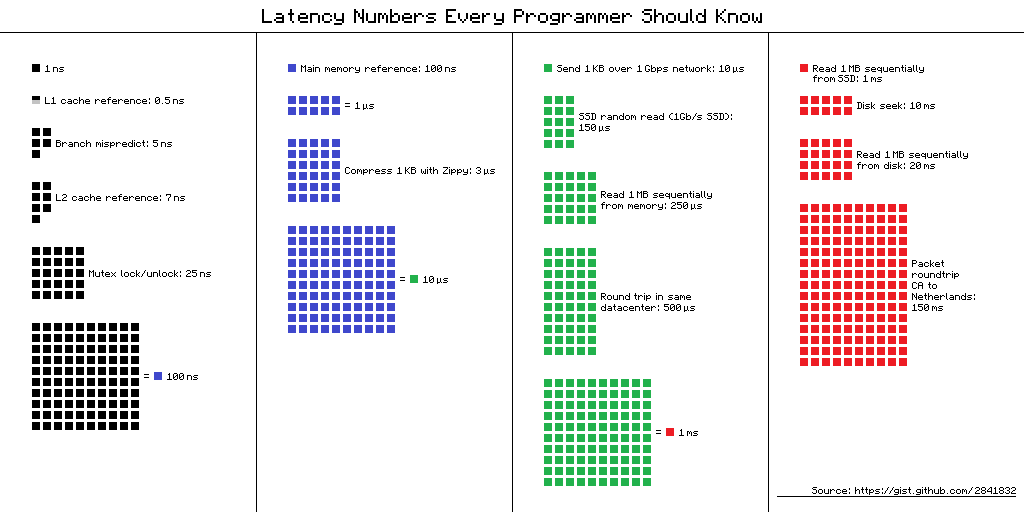
\includegraphics[width=\textwidth]{sources/appendices/images/latencies-refernece.png}
	\caption[]{Humanized visualization of the data in Table 
    \ref{tab:refernce_latencies}}.
	\label{fig:refernce_latencies}
\end{figure}

\FloatBarrier

\vspace{-2cm}
\section*{Data structures Asymptotic complexity cheatsheet}
% Please add the following required packages to your document preamble:
% \usepackage{booktabs}
% \usepackage{multirow}
% \usepackage{graphicx}
% \usepackage[table,xcdraw]{xcolor}
% If you use beamer only pass "xcolor=table" option, i.e. \documentclass[xcolor=table]{beamer}
\begin{table}[!htbp]
    \centering
    \resizebox{\textwidth}{!}{%
    \begin{tabular}{@{}lccccccccc@{}}
    \toprule
                                              & \multicolumn{8}{l}{\textbf{Time Complexities}}                                                                                                                                                                                                                                                                                                                                                  & \multicolumn{1}{l}{\textbf{Space Complexity}}             \\ \cmidrule(l){2-10} 
                                              & \multicolumn{1}{l}{\textbf{Average case}}    & \multicolumn{7}{l}{\textbf{Worst case}}                                                                                                                                                                                                                                                                                                          & \multicolumn{1}{l}{}                                      \\
    \multirow{-3}{*}{\textbf{Data Structure}} & \multicolumn{1}{l}{\textit{\textbf{Access}}} & \multicolumn{1}{l}{\textit{\textbf{Search}}} & \multicolumn{1}{l}{\textit{\textbf{Insertion}}} & \multicolumn{1}{l}{\textit{\textbf{Deletion}}} & \multicolumn{1}{l}{\textit{\textbf{Access}}} & \multicolumn{1}{l}{\textit{\textbf{Search}}} & \multicolumn{1}{l}{\textit{\textbf{Insertion}}} & \multicolumn{1}{l}{\textit{\textbf{Deletion}}} & \multicolumn{1}{l}{\multirow{-2}{*}{\textbf{Worst case}}} \\ \cmidrule(r){1-1}
    Array                                     & \cellcolor[HTML]{009901}$O(1)$               & \cellcolor[HTML]{FFC702}$O(n)$               & \cellcolor[HTML]{FFC702}$O(n)$                  & \cellcolor[HTML]{FFC702}$O(n)$                 & \cellcolor[HTML]{009901}$O(1)$               & \cellcolor[HTML]{FFC702}$O(n)$               & \cellcolor[HTML]{FFC702}$O(n)$                  & \cellcolor[HTML]{FFC702}$O(n)$                 & \cellcolor[HTML]{FFC702}$O(n)$                            \\
    Stack                                     & \cellcolor[HTML]{009901}$O(1)$               & \cellcolor[HTML]{656565}N.A.                 & \cellcolor[HTML]{009901}$O(1)$                  & \cellcolor[HTML]{009901}$O(1)$                 & \cellcolor[HTML]{009901}$O(1)$               & \cellcolor[HTML]{656565}N.A.                 & \cellcolor[HTML]{009901}$O(1)$                  & \cellcolor[HTML]{009901}$O(1)$                 & \cellcolor[HTML]{FFC702}$O(n)$                            \\
    Queue                                     & \cellcolor[HTML]{009901}$O(1)$               & \cellcolor[HTML]{656565}N.A.                 & \cellcolor[HTML]{009901}$O(1)$                  & \cellcolor[HTML]{009901}$O(1)$                 & \cellcolor[HTML]{009901}$O(1)$               & \cellcolor[HTML]{656565}N.A.                 & \cellcolor[HTML]{009901}$O(1)$                  & \cellcolor[HTML]{009901}$O(1)$                 & \cellcolor[HTML]{FFC702}$O(n)$                            \\
    Singly Linked List                        & \cellcolor[HTML]{FFC702}$O(n)$               & \cellcolor[HTML]{FFC702}$O(n)$               & \cellcolor[HTML]{009901}$O(1)$                  & \cellcolor[HTML]{FFC702}$O(n)$                 & \cellcolor[HTML]{FFC702}$O(n)$               & \cellcolor[HTML]{FFC702}$O(n)$               & \cellcolor[HTML]{009901}$O(1)$                  & \cellcolor[HTML]{FFC702}$O(n)$                 & \cellcolor[HTML]{FFC702}$O(n)$                            \\
    Doubly Linked List                        & \cellcolor[HTML]{FFC702}$O(n)$               & \cellcolor[HTML]{FFC702}$O(n)$               & \cellcolor[HTML]{009901}$O(1)$                  & \cellcolor[HTML]{009901}$O(1)$                 & \cellcolor[HTML]{FFC702}$O(n)$               & \cellcolor[HTML]{FFC702}$O(n)$               & \cellcolor[HTML]{009901}$O(1)$                  & \cellcolor[HTML]{009901}$O(1)$                 & \cellcolor[HTML]{FFC702}$O(n)$                            \\
    Hash Table                                & \cellcolor[HTML]{009901}$O(1)$               & \cellcolor[HTML]{009901}$O(1)$               & \cellcolor[HTML]{009901}$O(1)$                  & \cellcolor[HTML]{009901}$O(1)$                 & \cellcolor[HTML]{FFC702}$O(n)$               & \cellcolor[HTML]{FFC702}$O(n)$               & \cellcolor[HTML]{FFC702}$O(n)$                  & \cellcolor[HTML]{FFC702}$O(n)$                 & \cellcolor[HTML]{FFC702}$O(n)$                            \\
    Binary Search Tree                        & \cellcolor[HTML]{32CB00}$O(log_2(n))$        & \cellcolor[HTML]{32CB00}$O(log_2(n))$        & \cellcolor[HTML]{32CB00}$O(log_2(n))$           & \cellcolor[HTML]{32CB00}$O(log_2(n))$          & \cellcolor[HTML]{FFC702}$O(n)$               & \cellcolor[HTML]{FFC702}$O(n)$               & \cellcolor[HTML]{FFC702}$O(n)$                  & \cellcolor[HTML]{FFC702}$O(n)$                 & \cellcolor[HTML]{FFC702}$O(n)$                            \\
    Red-Black Tree                            & \cellcolor[HTML]{32CB00}$O(log_2(n))$        & \cellcolor[HTML]{32CB00}$O(log_2(n))$        & \cellcolor[HTML]{32CB00}$O(log_2(n))$           & \cellcolor[HTML]{32CB00}$O(log_2(n))$          & \cellcolor[HTML]{32CB00}$O(log_2(n))$        & \cellcolor[HTML]{32CB00}$O(log_2(n))$        & \cellcolor[HTML]{32CB00}$O(log_2(n))$           & \cellcolor[HTML]{32CB00}$O(log_2(n))$          & \cellcolor[HTML]{FFC702}$O(n)$                            \\
    Heap                                      & \cellcolor[HTML]{009901}$O(1)$               & \cellcolor[HTML]{656565}N.A.                 & \cellcolor[HTML]{32CB00}$O(log_2(n))$           & \cellcolor[HTML]{32CB00}$O(log_2(n))$          & \cellcolor[HTML]{009901}$O(1)$               & \cellcolor[HTML]{656565}N.A.                 & \cellcolor[HTML]{32CB00}$O(log_2(n))$           & \cellcolor[HTML]{32CB00}$O(log_2(n))$          & \cellcolor[HTML]{FFC702}$O(n)$                            \\ \bottomrule
    \end{tabular}%
    }
    \caption{Asymptotic complexities for a number of data strucutes. For time, both the average and case is reported, while for space only the worst. $O(1) < O(log_2(n)) < O(log_2(n)) < O(n) < O(nlog_2(n) < O(n^2) < O(n^3) \ldots < O(2^n) < O(n!) < O(n^n)$  }
    \label{appendix:ds_complexities}
\end{table}


\begin{figure}
    \centering
\begin{tikzpicture}
    \begin{axis}[
      grid = major,
      clip = true,
      ticks = none,
      width=0.9\textwidth,
      height=0.7\textwidth,
      every axis plot/.append style={very thick},
      axis line style = ultra thick,
      clip mode=individual,
      restrict y to domain=0:40,
      restrict x to domain=0:20,
      axis x line = left,
      axis y line = left,
      domain = 0.00:10,
      xmin = 0,
      xmax = 11,
      ymin = 0,
      ymax = 42,
      xlabel = n,
      ylabel = no. of operations,
      xlabel style = {at={(axis description cs:0.5,-0.1)},anchor=south},
      ylabel style = {at={(axis description cs:-0.08,0.5)},anchor=north},
      label style = {font=\LARGE\bf},
    ]
  \addplot [
      samples=100, 
      color=red,
  ]
  {x^2}node[above,pos=1,style={font=\Large}]{$\mathcal{O}(n^2)$};
  \addplot [
      samples=100, 
      color=blue,
  ]
  {x}node[above,pos=1,style={font=\Large}]{$\mathcal{O}(n)$};
  \addplot [
      samples=100, 
      color=orange,
  ]
  {log2 x}node[above,pos=1,style={font=\Large}]{$\mathcal{O}(\log{}n)$};
  \addplot [
      samples=100, 
      color=black,
  ]
  {x*(log2 x)}node[above,pos=1,style={font=\Large}]{$\mathcal{O}(n\log{}n)$};
  \addplot [
      samples=100, 
      color=magenta,
  ]
  {1}node[above,pos=1,style={font=\Large}]{$\mathcal{O}(1)$};
  \addplot [
      samples=100, 
      color=cyan,
  ]
  {x^(2.2)}node[above,pos=1,style={font=\Large}]{$\mathcal{O}(n^3)$};
  

  \addplot [
    samples=100,
    color=green, 
  ] gnuplot{gamma(x+3)} node[above,pos=1,style={font=\Large}]{$\mathcal{O}(n!)$};

  \addplot [
    samples=100, 
    color=yellow,
]
{2.5*2^x}node[above,pos=1,style={font=\Large}]{$\mathcal{O}(2^x)$};
  
  \end{axis}
  \end{tikzpicture}

  \caption[]{Graph showing the relative growth rates of common function used to describe algorithms.}
  \label{fig:ds_complexities:graph}
\end{figure}
%%%%%%%%%%%%%%%%%%%%%%%%%%%%%%%%%%%%%%%%%%%%
%               BIBLIOGRAPHY
%%%%%%%%%%%%%%%%%%%%%%%%%%%%%%%%%%%%%%%%%%%%

%
%from documentation
%\newacronym[⟨key-val list⟩]{⟨label ⟩}{⟨abbrv ⟩}{⟨long⟩}
%above is short version of this
% \newglossaryentry{⟨label ⟩}{type=\acronymtype,
% name={⟨abbrv ⟩},
% description={⟨long⟩},
% text={⟨abbrv ⟩},
% first={⟨long⟩ (⟨abbrv ⟩)},
% plural={⟨abbrv ⟩\glspluralsuffix},
% firstplural={⟨long⟩\glspluralsuffix\space (⟨abbrv ⟩\glspluralsuffix)},
% ⟨key-val list⟩}

\newacronym{cd}{CD}{compact disk}
\newacronym{utc}{UTC}{Coordinated Universal Time}
%\newacronym{adt}{ADT}{Atlantic Daylight Time}
%\newacronym{est}{EST}{Eastern Standard Time}
 
% Use the acronyms
\gls{utc} is 3 hours behind \gls{adt} and 10 hours ahead of \gls{est}.



%\addcontentsline{toc}{chapter}{\textcolor{ocre}{Glossary}}
%\printglossaries


%Print the glossary

\addcontentsline{toc}{chapter}{\textcolor{ocre}{Bibliography}}
%\chapter*{Bibliography}
%Print the glossary
\printbibliography	
	
%%%%%%%%%%%%%%%%%%%%%%%%%%%%%%%%%%%%%%%%%%%%
%               INDEX
%%%%%%%%%%%%%%%%%%%%%%%%%%%%%%%%%%%%%%%%%%%%	
	\cleardoublepage
	\phantomsection
	\setlength{\columnsep}{0.75cm}
	\addcontentsline{toc}{chapter}{\textcolor{ocre}{Index}}
	\printindex


	%\backmatter

\end{document}
